%--------------------------------------------------
\subsection{Optical~Character~Recognition}
\label{subsec:ocr}
%--------------------------------------------------

When it comes to \ac{OCR} we experimented with different methods. Our first
approach followed the architecture published by \cite{7801919}.  Unfortunately
at the end of the development cycle we had to use a different model, because the
original method did not provide the desired results.  In the final solution we
utilize the \emph{paddleOCR} system by \cite{DBLP:journals/corr/abs-2009-09941}.
Nevertheless we wanted to describe the original method proposed by
\cite{7801919}, since this was in the focus of our development efforts for the
majority of the project. Thus, the following section serves as a brief
introduction to an otherwise promising \ac{OCR} architecture.

\begin{figure}
	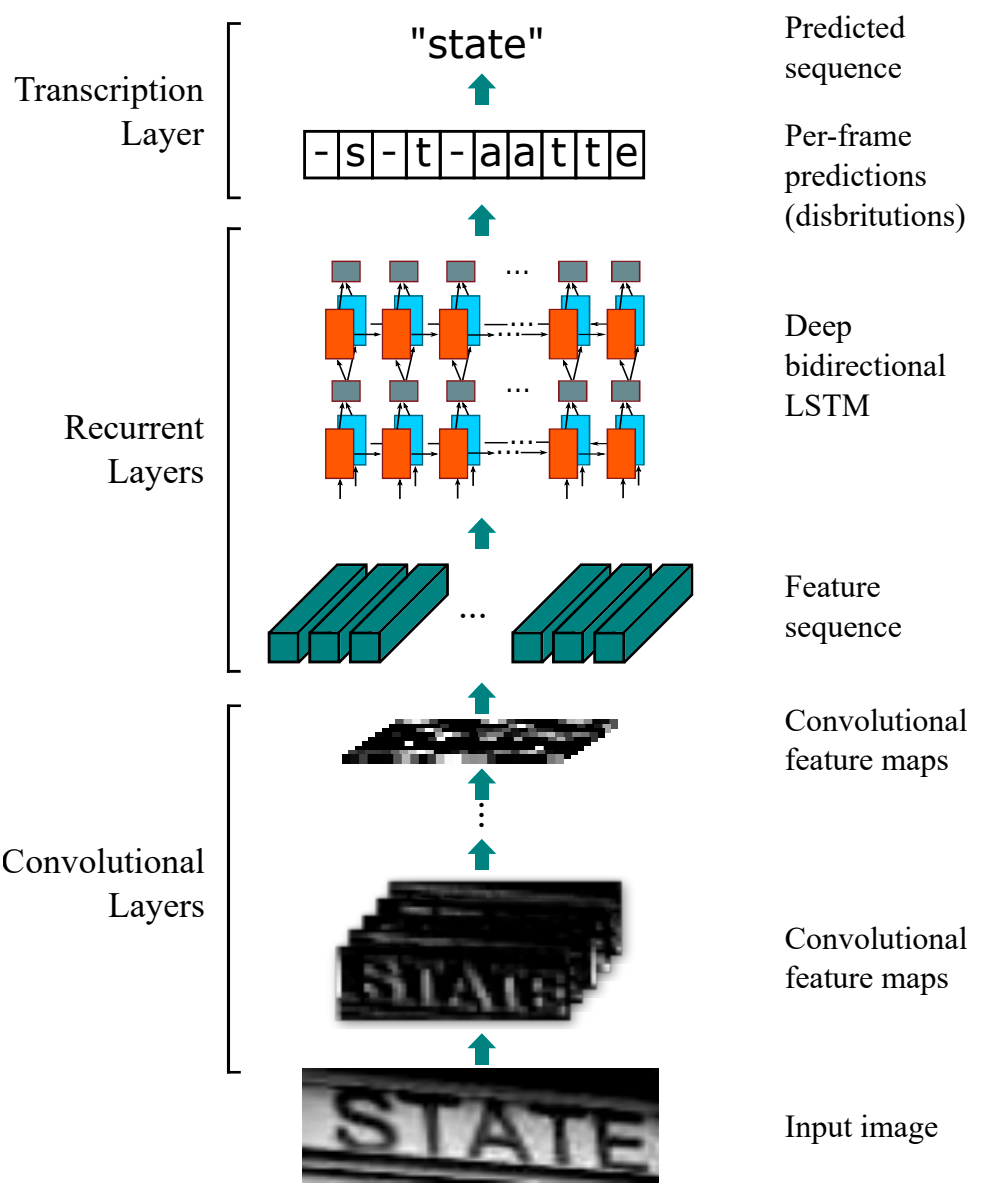
\includegraphics[width=\textwidth]{figures/crnn.png}
	\caption{The architecture published in \cite{7801919}}
	\label{fig:ocr_architecture}
\end{figure}

We deal with the classic problem of computer vision, image-based sequence
recognition. Serial objects, such as scene text, are usually recognized as
a sequence of tags rather than a single tag. RNNs can be trained and optimized
end-to-end, but require complex post-processing steps before being used. CRNN is
a combination of DCNN and RNN and forms an end-to-end system for sequence
recognition. It can be learned directly from sequence labels, does not require
detailed annotations (such as words), and only requires height normalization in
the training and testing sessions.

A CRNN is a type of Recurrent Neural Network (RNN) that can be trained to make
a prediction for each frame of a sequence of features that is output by
convolutional layers. In CRNN, each column of the field maps corresponds to
a region of a rectangle (called the receptive field) of the original image, and
the regions are in the same order as the corresponding columns in the feature
maps from left to right. A deep bidirectional recurrent neural network (CRNN) is
built on top of convolutional layers as recurrent layers.

The recurrent layers predict a label distribution $y_t$ for each frame $x_t$ of
the feature sequence. Each time it receives a frame in the sequence, it updates
its internal state with a non-linear function that takes both the current input
state and the past state as input. Long-Short-Term Memory (LSTM) is a type of
RNN designed to capture long-range dependencies that often occur in image-based
sequences. LSTM consists of a memory cell and three multiplicative gates, namely
input, output and forget gates. It has made a huge improvement in its speech
recognition function.  Transcription is a process that produces frame-by-frame
predictions into a tag sequence using RNN. Each input in CTC is a sequence $y
= y_1, \dots , y_T$, where $T$ is the length of the sequence.

We have developed a neural network that can be trained end-to-end on pairs of
images, eliminating the manual labeling of individual components on the training
images. The network is trained with error differences calculated using the
backpropagation algorithm and stochastic gradient descent (SGD).  CRNN is not
limited to recognizing a word in a known dictionary and can handle random
strings, sentences or other scripts.  The recognition accuracy is plotted as
a function of $d$. A larger $d$ results in more candidates, thus a more accurate
lexicon-based transcription. On the other hand, the computational cost increases
with larger $d$, due to the longer BKtree search time. CRNN outperforms
commercial OMR engines such as Capella Scan and PhotoScore by a wide margin.

CRNN uses convolutional features that are highly robust against noise and bias.
It can be easily applied to other image-based sequence recognition
probabilities, requiring minimal domain knowledge.  CRNN, a new neural network
architecture that integrates the advantages of both deep convolutional neural
networks and recurrent neural networks. It runs directly on coarse-level labels
(such as words) and does not require detailed annotations for each eleventh
(i.e., character) in the training phase.
